\section{Marco teórico}\label{sec:teoria}
\subsection{Continuidad y condición de unión}
Para flujo permanente e incompresible, sin almacenamiento en el nodo, $Q_0=Q_1+Q_2$. Se denota la fracción derivada al ramal 2 por $\varphi=Q_2/Q_0$. El régimen local se caracteriza por el número de Froude $Fr=V/\sqrt{gD}$, con $D=A/T$; para una sección rectangular $D=y$. Se adopta $z_J$ como cota de solera común en la unión, y las dos ramas comparten en la sección de unión el nivel de superficie libre $H_J=z_J+y_J$, sin que ello implique igualdad de velocidades ni de cargas totales.

\subsection{Formulación I: flujo plano ideal con tapa rígida}\label{sec:f1}
Como cierre independiente de la energía y de la fricción, una bifurcación puede idealizarse como flujo plano, permanente, irrotacional y no viscoso, con superficie libre aproximada por una tapa rígida (límite de $Fr$ pequeño). Con el potencial complejo $w=\phi+i\psi$ y la geometría poligonal, el mapeo de Schwarz--Christoffel conduce a la solución de Milne-Thomson para paredes semiinfinitas \citep[\S 10.8]{milnethomson1962}; véase también \citet{batchelor1967} y \citet{gurevich1965}. Sean $\lambda=b_1/b_0$ y $\mu=b_2/b_0$ las relaciones de ancho, $u_i=U_i/U$ las velocidades lejanas adimensionales y $e=1-\pi/\alpha$ (con $0<\alpha<\pi$ el ángulo de la derivación). La continuidad y la condición de estancamiento en la esquina aguas abajo dan
\begin{equation}
\lambda u_1+\mu u_2=1,\qquad \lambda u_1^{\,e}-\mu u_2^{\,e}=1,\qquad \varphi=\mu u_2.
\label{eq:f1}
\end{equation}
La Figura~\ref{fig:mapeo} esquematiza el dominio físico y la red de flujo. Esta formulación no contiene rugosidad, longitud ni condición aguas abajo; por tanto, \emph{fija el reparto solo con la geometría}. Para que un canal real cumpla la solución, los ramales tendrían que desarrollar niveles distintos (tirantes menores en el ramal con mayor velocidad), diferencia que la solución ideal no limita.

\begin{figure}[htbp]
\centering
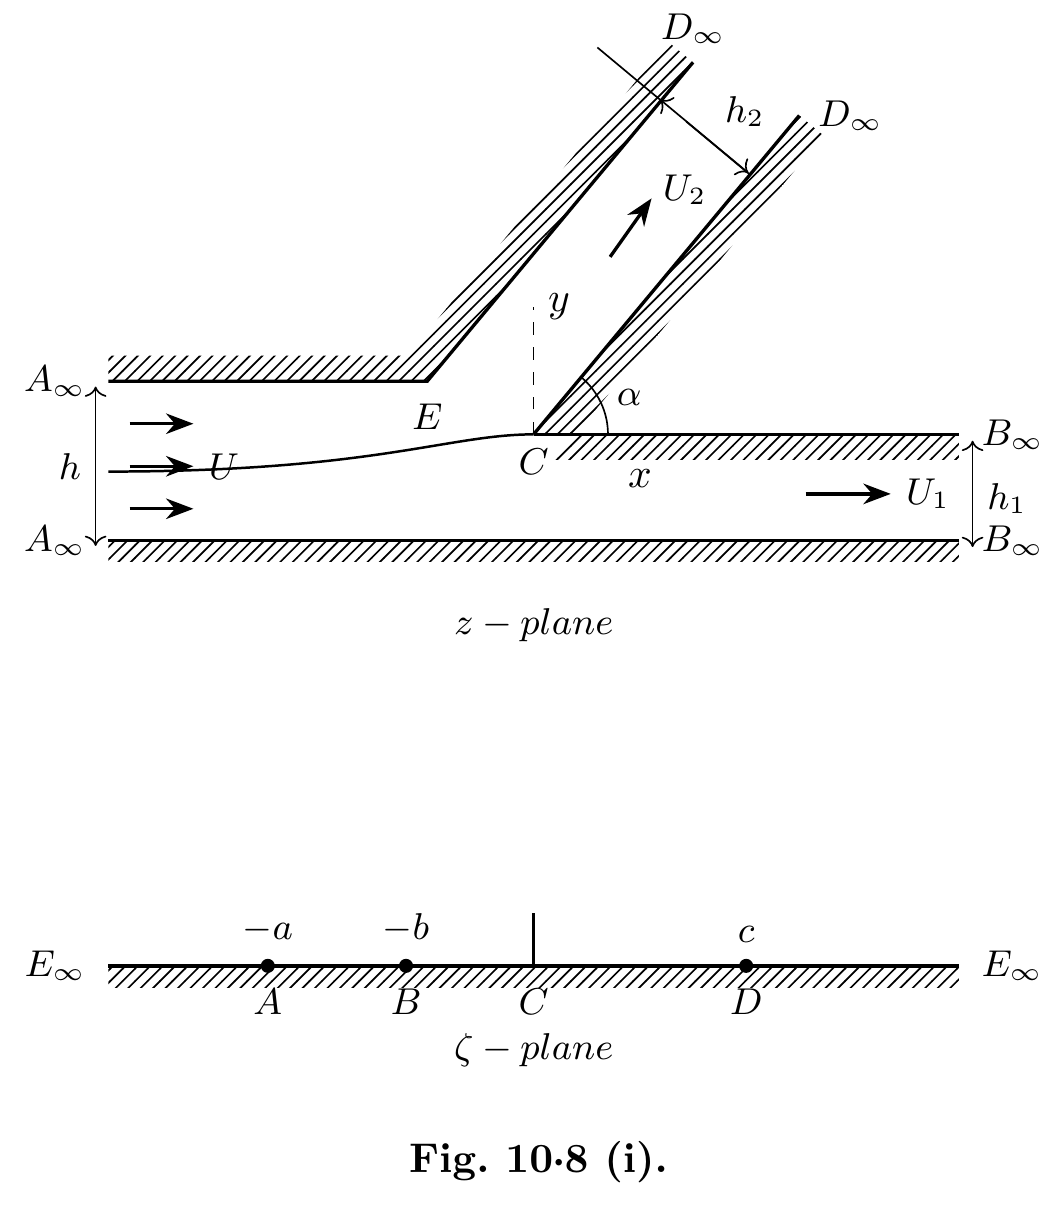
\includegraphics[width=0.62\linewidth]{1.png}
\caption{Flujo plano en una bifurcación de canal y planos $z$ y $\zeta$ del mapeo conforme.}
\label{fig:mapeo}
\Fuente{Reproducido de \citet{milnethomson1962}.}
\end{figure}

\subsection{Formulación II: energía por ramal con nivel común}\label{sec:f2}
La Formulación II sigue la ecuación de energía entre la unión y una sección terminal de cada ramal, con unión de redes tipo \citet[cap.~6]{chaudhry2008}. Para un ramal rectangular $i$ de ancho $b_i$,
\begin{equation}
G_i=H_J+(1-K_i)\frac{Q_i^2}{2gA_{J,i}^2}-(z_{d,i}+y_{d,i})-\frac{Q_i^2}{2gA_{d,i}^2}-\frac{L_i}{2}\!\left[S_{f,i}(Q_i,y_J)+S_{f,i}(Q_i,y_{d,i})\right]=0,
\label{eq:Gi}
\end{equation}
con $A_{J,i}=b_iy_J$, $A_{d,i}=b_iy_{d,i}$, $z_{d,i}=z_J-S_iL_i$, $K_i$ el coeficiente de pérdida local aplicado a la carga cinética nodal y $S_f=\left(nQ/AR^{2/3}\right)^2$ la pendiente de fricción de Manning, con $R=A/P=b_iy/(b_i+2y)$. La fricción se integra con la regla del trapecio entre los dos tirantes extremos; no se resuelve el perfil $y(x)$.

Las incógnitas son $\mathbf X=[Q_1,Q_2,H_J]^{\mathsf T}$ y el sistema normalizado es
\begin{equation}
\mathbf F(\mathbf X)=\begin{bmatrix}(Q_0-Q_1-Q_2)/Q_0\\ G_1(Q_1,H_J)/y_{\mathrm{ref}}\\ G_2(Q_2,H_J)/y_{\mathrm{ref}}\end{bmatrix}=\mathbf 0,\qquad
\mathbf J=\begin{bmatrix}-1/Q_0&-1/Q_0&0\\ G_{1,Q}/y_{\mathrm{ref}}&0&G_{1,H}/y_{\mathrm{ref}}\\ 0&G_{2,Q}/y_{\mathrm{ref}}&G_{2,H}/y_{\mathrm{ref}}\end{bmatrix},
\label{eq:sistema}
\end{equation}
con $y_{\mathrm{ref}}=1.60$ m. El ángulo $\theta$ no aparece en las ecuaciones \eqref{eq:Gi}--\eqref{eq:sistema}: con parámetros de sección, rugosidad, longitud, pendiente y calados fijos, la formulación predice el mismo reparto para todo $\theta$. Es una propiedad del modelo y no evidencia de que el ángulo carezca de efecto físico. Para dimensionar un ramal se puede añadir $b_2$ como incógnita y la restricción $Q_2=\varphi_\ast Q_0$, lo que da un sistema $4\times4$ con la misma estructura.

\subsection{Método de Newton--Raphson}
Dado $\mathbf X^{(k)}$, el paso se obtiene de $\mathbf J(\mathbf X^{(k)})\,\Delta\mathbf X=-\mathbf F(\mathbf X^{(k)})$ y la actualización $\mathbf X^{(k+1)}=\mathbf X^{(k)}+\alpha_k\Delta\mathbf X$ usa un factor de amortiguación $\alpha_k\in(0,1]$ por retroceso hasta que $\|\mathbf F\|$ decrezca \citep{chapra2015}. Con jacobiano analítico y buen punto inicial la convergencia es cuadrática cerca de la raíz. La convergencia desde un punto dado no demuestra existencia ni unicidad de la solución física.

\subsection{Sensibilidad local e incertidumbre paramétrica}
Si $\mathbf F(\mathbf X^\ast,\mathbf p)=\mathbf 0$, la diferenciación implícita da
\begin{equation}
\frac{\partial\mathbf X^\ast}{\partial p_k}=-\mathbf J^{-1}\frac{\partial\mathbf F}{\partial p_k},\qquad
E_{\varphi,p_k}=\frac{\partial\varphi}{\partial p_k}\frac{p_k}{\varphi},
\label{eq:elast}
\end{equation}
donde $E$ es la elasticidad local. Con parámetros independientes de desviación $\sigma_{p_k}$, la varianza lineal es $\sigma_\varphi^2\simeq\sum_k(\partial\varphi/\partial p_k\,\sigma_{p_k})^2$, que se contrasta con una simulación Monte Carlo \citep{saltelli2008}. Ambas son condicionales a las desviaciones postuladas y no son intervalos de confianza del desempeño real.

\subsection{Modelo 2D de HEC-RAS: ecuaciones de aguas poco profundas}\label{sec:dw}
Las ecuaciones 2D de Saint-Venant promediadas en profundidad expresan continuidad y cantidad de movimiento para el tirante $d$ y las velocidades medias $u,v$:
\begin{align}
\partial_t d+\partial_x(du)+\partial_y(dv)&=q_s,\nonumber\\
\partial_t(du)+\partial_x\!\left(du^2+\tfrac12gd^2\right)+\partial_y(duv)&=-gd\,\partial_xz_b-\tau_{b,x}/\rho,
\label{eq:swe}
\end{align}
y una ecuación análoga en $y$. HEC-RAS ofrece este sistema con dos tratamientos numéricos, SWE-ELM y SWE-EM (este último con un tratamiento más estricto de la cantidad de movimiento), además de una \emph{onda difusiva} que desprecia la aceleración local y convectiva \citep{hecmomentum,hecmanual}. En este trabajo se usa SWE-EM, elegido porque reproduce el remanso 1D en ramales angostos y diagonales (Sección~\ref{sec:verif2d}). En el formulario 2D el radio hidráulico se aproxima por el tirante local ($R\approx d$), de modo que la rugosidad efectiva de una sección angosta difiere de la que aplica un modelo 1D con perímetro mojado completo. Para medir la resistencia que el modelo produce realmente se define la rugosidad efectiva
\begin{equation}
n_\mathrm{eff}=\frac{A\,R^{2/3}\sqrt{S_f}}{Q},
\label{eq:neff}
\end{equation}
con $S_f$ la pendiente de la línea de energía simulada ($E=\zeta+V^2/2g$) entre el 15 y el 85\pc de la longitud del ramal; $n_\mathrm{eff}$ difiere del $n$ ingresado cuando la discretización añade o quita resistencia.

\subsection{Criterios de comparación}\label{sec:sesgo}
La fracción $\varphi_{2D}=Q_{2,2D}/Q_{0}$ y el error del reparto se definen por $\Delta\varphi=\varphi_{1D}-\varphi_{2D}$ y $\varepsilon(Q_2)=100\,(Q_{2,1D}-Q_{2,2D})/Q_{2,2D}$. Como referencia operativa se adoptan los umbrales de $\varepsilon(Q_2)\leq10\pc$ (aceptable) y $\leq20\pc$ (marginal), propuestos por el grupo y pendientes de confirmación por el docente; no son una norma. La verificación del modelo 2D usa una tolerancia de $\pm0.01$ m en el nivel del agua respecto del remanso 1D.
